\documentclass[journal]{IEEEtran}
%
% If IEEEtran.cls has not been installed into the LaTeX system files,
% manually specify the path to it like:
% \documentclass[journal]{../sty/IEEEtran}

% Some very useful LaTeX packages include:
% (uncomment the ones you want to load)


% *** MISC UTILITY PACKAGES ***
%
%\usepackage{ifpdf}
% Heiko Oberdiek's ifpdf.sty is very useful if you need conditional
% compilation based on whether the output is pdf or dvi.
% usage:
% \ifpdf
%   % pdf code
% \else
%   % dvi code
% \fi
% The latest version of ifpdf.sty can be obtained from:
% http://www.ctan.org/pkg/ifpdf
% Also, note that IEEEtran.cls V1.7 and later provides a builtin
% \ifCLASSINFOpdf conditional that works the same way.
% When switching from latex to pdflatex and vice-versa, the compiler may
% have to be run twice to clear warning/error messages.

\usepackage{listings}

% *** CITATION PACKAGES ***
%
%\usepackage{cite}
% cite.sty was written by Donald Arseneau
% V1.6 and later of IEEEtran pre-defines the format of the cite.sty package
% \cite{} output to follow that of the IEEE. Loading the cite package will
% result in citation numbers being automatically sorted and properly
% "compressed/ranged". e.g., [1], [9], [2], [7], [5], [6] without using
% cite.sty will become [1], [2], [5]--[7], [9] using cite.sty. cite.sty's
% \cite will automatically add leading space, if needed. Use cite.sty's
% noadjust option (cite.sty V3.8 and later) if you want to turn this off
% such as if a citation ever needs to be enclosed in parenthesis.
% cite.sty is already installed on most LaTeX systems. Be sure and use
% version 5.0 (2009-03-20) and later if using hyperref.sty.
% The latest version can be obtained at:
% http://www.ctan.org/pkg/cite
% The documentation is contained in the cite.sty file itself.

% *** GRAPHICS RELATED PACKAGES ***
%
\ifCLASSINFOpdf
  \usepackage[pdftex]{graphicx}
  % declare the path(s) where your graphic files are
  % \graphicspath{{../pdf/}{../jpeg/}}
  % and their extensions so you won't have to specify these with
  % every instance of \includegraphics
  % \DeclareGraphicsExtensions{.pdf,.jpeg,.png}
\else
  % or other class option (dvipsone, dvipdf, if not using dvips). graphicx
  % will default to the driver specified in the system graphics.cfg if no
  % driver is specified.
  % \usepackage[dvips]{graphicx}
  % declare the path(s) where your graphic files are
  % \graphicspath{{../eps/}}
  % and their extensions so you won't have to specify these with
  % every instance of \includegraphics
  % \DeclareGraphicsExtensions{.eps}
\fi
% graphicx was written by David Carlisle and Sebastian Rahtz. It is
% required if you want graphics, photos, etc. graphicx.sty is already
% installed on most LaTeX systems. The latest version and documentation
% can be obtained at: 
% http://www.ctan.org/pkg/graphicx
% Another good source of documentation is "Using Imported Graphics in
% LaTeX2e" by Keith Reckdahl which can be found at:
% http://www.ctan.org/pkg/epslatex
%
% latex, and pdflatex in dvi mode, support graphics in encapsulated
% postscript (.eps) format. pdflatex in pdf mode supports graphics
% in .pdf, .jpeg, .png and .mps (metapost) formats. Users should ensure
% that all non-photo figures use a vector format (.eps, .pdf, .mps) and
% not a bitmapped formats (.jpeg, .png). The IEEE frowns on bitmapped formats
% which can result in "jaggedy"/blurry rendering of lines and letters as
% well as large increases in file sizes.
%
% You can find documentation about the pdfTeX application at:
% http://www.tug.org/applications/pdftex

% *** MATH PACKAGES ***
%
\usepackage{amsmath}
% A popular package from the American Mathematical Society that provides
% many useful and powerful commands for dealing with mathematics.
%
% Note that the amsmath package sets \interdisplaylinepenalty to 10000
% thus preventing page breaks from occurring within multiline equations. Use:
%\interdisplaylinepenalty=2500
% after loading amsmath to restore such page breaks as IEEEtran.cls normally
% does. amsmath.sty is already installed on most LaTeX systems. The latest
% version and documentation can be obtained at:
% http://www.ctan.org/pkg/amsmath


% *** SUBFIGURE PACKAGES ***
\ifCLASSOPTIONcompsoc
  \usepackage[caption=false,font=normalsize,labelfont=sf,textfont=sf]{subfig}
\else
  \usepackage[caption=false,font=footnotesize]{subfig}
\fi
% subfig.sty, written by Steven Douglas Cochran, is the modern replacement
% for subfigure.sty, the latter of which is no longer maintained and is
% incompatible with some LaTeX packages including fixltx2e. However,
% subfig.sty requires and automatically loads Axel Sommerfeldt's caption.sty
% which will override IEEEtran.cls' handling of captions and this will result
% in non-IEEE style figure/table captions. To prevent this problem, be sure
% and invoke subfig.sty's "caption=false" package option (available since
% subfig.sty version 1.3, 2005/06/28) as this is will preserve IEEEtran.cls
% handling of captions.
% Note that the Computer Society format requires a larger sans serif font
% than the serif footnote size font used in traditional IEEE formatting
% and thus the need to invoke different subfig.sty package options depending
% on whether compsoc mode has been enabled.
%
% The latest version and documentation of subfig.sty can be obtained at:
% http://www.ctan.org/pkg/subfig




% *** FLOAT PACKAGES ***
%
%\usepackage{fixltx2e}
% fixltx2e, the successor to the earlier fix2col.sty, was written by
% Frank Mittelbach and David Carlisle. This package corrects a few problems
% in the LaTeX2e kernel, the most notable of which is that in current
% LaTeX2e releases, the ordering of single and double column floats is not
% guaranteed to be preserved. Thus, an unpatched LaTeX2e can allow a
% single column figure to be placed prior to an earlier double column
% figure.
% Be aware that LaTeX2e kernels dated 2015 and later have fixltx2e.sty's
% corrections already built into the system in which case a warning will
% be issued if an attempt is made to load fixltx2e.sty as it is no longer
% needed.
% The latest version and documentation can be found at:
% http://www.ctan.org/pkg/fixltx2e


%\usepackage{stfloats}
% stfloats.sty was written by Sigitas Tolusis. This package gives LaTeX2e
% the ability to do double column floats at the bottom of the page as well
% as the top. (e.g., "\begin{figure*}[!b]" is not normally possible in
% LaTeX2e). It also provides a command:
%\fnbelowfloat
% to enable the placement of footnotes below bottom floats (the standard
% LaTeX2e kernel puts them above bottom floats). This is an invasive package
% which rewrites many portions of the LaTeX2e float routines. It may not work
% with other packages that modify the LaTeX2e float routines. The latest
% version and documentation can be obtained at:
% http://www.ctan.org/pkg/stfloats
% Do not use the stfloats baselinefloat ability as the IEEE does not allow
% \baselineskip to stretch. Authors submitting work to the IEEE should note
% that the IEEE rarely uses double column equations and that authors should try
% to avoid such use. Do not be tempted to use the cuted.sty or midfloat.sty
% packages (also by Sigitas Tolusis) as the IEEE does not format its papers in
% such ways.
% Do not attempt to use stfloats with fixltx2e as they are incompatible.
% Instead, use Morten Hogholm'a dblfloatfix which combines the features
% of both fixltx2e and stfloats:
%
% \usepackage{dblfloatfix}
% The latest version can be found at:
% http://www.ctan.org/pkg/dblfloatfix


%\ifCLASSOPTIONcaptionsoff
%  \usepackage[nomarkers]{endfloat}
% \let\MYoriglatexcaption\caption
% \renewcommand{\caption}[2][\relax]{\MYoriglatexcaption[#2]{#2}}
%\fi
% endfloat.sty was written by James Darrell McCauley, Jeff Goldberg and 
% Axel Sommerfeldt. This package may be useful when used in conjunction with 
% IEEEtran.cls'  captionsoff option. Some IEEE journals/societies require that
% submissions have lists of figures/tables at the end of the paper and that
% figures/tables without any captions are placed on a page by themselves at
% the end of the document. If needed, the draftcls IEEEtran class option or
% \CLASSINPUTbaselinestretch interface can be used to increase the line
% spacing as well. Be sure and use the nomarkers option of endfloat to
% prevent endfloat from "marking" where the figures would have been placed
% in the text. The two hack lines of code above are a slight modification of
% that suggested by in the endfloat docs (section 8.4.1) to ensure that
% the full captions always appear in the list of figures/tables - even if
% the user used the short optional argument of \caption[]{}.
% IEEE papers do not typically make use of \caption[]'s optional argument,
% so this should not be an issue. A similar trick can be used to disable
% captions of packages such as subfig.sty that lack options to turn off
% the subcaptions:
% For subfig.sty:
% \let\MYorigsubfloat\subfloat
% \renewcommand{\subfloat}[2][\relax]{\MYorigsubfloat[]{#2}}
% However, the above trick will not work if both optional arguments of
% the \subfloat command are used. Furthermore, there needs to be a
% description of each subfigure *somewhere* and endfloat does not add
% subfigure captions to its list of figures. Thus, the best approach is to
% avoid the use of subfigure captions (many IEEE journals avoid them anyway)
% and instead reference/explain all the subfigures within the main caption.
% The latest version of endfloat.sty and its documentation can obtained at:
% http://www.ctan.org/pkg/endfloat
%
% The IEEEtran \ifCLASSOPTIONcaptionsoff conditional can also be used
% later in the document, say, to conditionally put the References on a 
% page by themselves.




% *** PDF, URL AND HYPERLINK PACKAGES ***
%
%\usepackage{url}
% url.sty was written by Donald Arseneau. It provides better support for
% handling and breaking URLs. url.sty is already installed on most LaTeX
% systems. The latest version and documentation can be obtained at:
% *** Do not adjust lengths that control margins, column widths, etc. ***
% *** Do not use packages that alter fonts (such as pslatex).         ***
% There should be no need to do such things with IEEEtran.cls V1.6 and later.
% (Unless specifically asked to do so by the journal or conference you plan
% to submit to, of course. )

\usepackage{tikz}
\usetikzlibrary{shapes.geometric, arrows, calc}
\tikzstyle{startstop} = [rectangle, rounded corners, minimum width=3cm, minimum height=0.5cm,text centered, draw=black, fill=white!30, ]
\tikzstyle{process} = [rectangle, minimum width=3cm, minimum height=0.5cm, text centered, draw=black, fill=white!30]
\tikzstyle{decision} = [diamond, minimum width=3cm, minimum height=1cm, text centered, draw=black, fill=green!30]
\tikzstyle{arrow} = [thick,->,>=stealth]

\usepackage{hyperref}

\begin{document}
%
% paper title
% Titles are generally capitalized except for words such as a, an, and, as,
% at, but, by, for, in, nor, of, on, or, the, to and up, which are usually
% not capitalized unless they are the first or last word of the title.
% Linebreaks \\ can be used within to get better formatting as desired.
% Do not put math or special symbols in the title.
\title{Motion Detection System Report}
%
%
% author names and IEEE memberships
% note positions of commas and nonbreaking spaces ( ~ ) LaTeX will not break
% a structure at a ~ so this keeps an author's name from being broken across
% two lines.
% use \thanks{} to gain access to the first footnote area
% a separate \thanks must be used for each paragraph as LaTeX2e's \thanks
% was not built to handle multiple paragraphs
%

\author{Joey Hines}

% The paper headers
\markboth{ELEC 7540: Digital Image Processing Report}%
{Shell \MakeLowercase{\textit{et al.}}: ELEC 7540: Digital Image Processing Report}


% make the title area
\maketitle

% As a general rule, do not put math, special symbols or citations
% in the abstract or keywords.
\begin{abstract}
As surveillance camera solutions have become cheaper, there are more video sources than ever to monitor
for surveillance. This report describes an algorithm and its implementation to detect motion in video sources.
The algorithm is designed to be simple and easy to implement. An implementation of the algorithm is also
presented with an analysis of its performance and results. 
\end{abstract}


% For peer review papers, you can put extra information on the cover
% page as needed:
% \ifCLASSOPTIONpeerreview
% \begin{center} \bfseries EDICS Category: 3-BBND \end{center}
% \fi
%
% For peerreview papers, this IEEEtran command inserts a page break and
% creates the second title. It will be ignored for other modes.
\IEEEpeerreviewmaketitle


\section{Introduction}
\IEEEPARstart{V}{ideo} surveillance has become more affordable in the last several years as costs of camera 
sensors and processors have dropped. With more video cameras than ever, it is important to be able to sift 
through video of nothing to find frames on interests. Commonly, this is done with motion detection. Frames of 
video are analyzed to determine if motion has
occurred in the video. 

This detection algorithm needs to be sensitive to motion and ideally not be set off by false alarms such as 
changes in light or dynamic objects within the scene. Consumers also expect camera units to be all-in-one. 
Meaning each camera should handle storing video and analyzing it for motion. As these cameras also need to be 
inexpensive, that often means cheaper  and less advanced processors are used. The challenge then becomes marking 
a motion detection algorithm that is lightweight enough to run on a cheaper processor and good enough to not set 
off false alarms. This report first explains an algorithm to preform motion detection.
Then, its implementation is discussed followed by a performance analysis and discussion on improvements. 

\section{Implemented Algorithm}
\label{section:algorithm}
The implemented algorithm was designed to be straight forward to implement while being useful for motion
detection. Figure \ref{fig:algorithm} shows the flowchart of the algorithm. The rest of this sections 
explains further each step and shares some of their implementation details. The full implemented code
can be found in Appendix \ref{appendix:code}.

\begin{figure}[!t]
    \centering
    \caption{Implemented Algorithm}
    \label{fig:algorithm}
    \begin{tikzpicture}[node distance=1cm]
        \node (start) [startstop] {Video Sequence};
        \node (bg_model) [process, below of=start] {Build Background Model};
        \node (bg_sub) [process, below of=bg_model] {Subtract Out Background};
        \node (motion_mask) [process, below of=bg_sub] {Apply Motion Mask};
        \node (threshold) [process, below of=motion_mask] {Threshold};
        \node (filter) [process, below of=threshold] {Apply Gaussian Filter};
        \node (median_filter) [process, below of= filter] {Apply Median Filter};
        \node (draw_box) [process, below of=median_filter] {Draw Motion Box};
        \node (update_bg_model) [process, below of=draw_box] {Update BG Model/Motion Mask};
        \node (display) [process, below of= update_bg_model] {Display output};
        \coordinate (flow) at ($(display.east)+(1.2cm,0)$);
        
        \draw [arrow] (start) -- (bg_model);
        \draw [arrow] (bg_model) -- (bg_sub);
        \draw [arrow] (bg_sub) -- (motion_mask);
        \draw [arrow] (motion_mask) -- (threshold);
        \draw [arrow] (threshold) -- (filter);
        \draw [arrow] (filter) -- (median_filter);
        \draw [arrow] (median_filter) -- (draw_box);
        \draw [arrow] (draw_box) -- (update_bg_model);
        \draw [arrow] (update_bg_model) -- (display);
        \draw [arrow] (display) -- (flow) |-  (bg_sub);
    \end{tikzpicture}
\end{figure}

\subsection{Video Sequence}
The algorithm is feed a series of frames from a video source. Frames can either be acquired from a Video For
Linux (VFL) capture device, such as a webcam, or be feed in from a sequence of image files. 
The latter is especially useful for testing, the testing process is further explored in Section 
\ref{section:program}. Live video capture is done by first initializing the V4L capture device. A separate
thread then handles gathering frames from the video source. When a new frame is available, the main thread
is notified and processes the frame. 

\subsubsection{Color System}
Many V4L sources use the the YUYV color system to capture video. YUYV is fully explained in \cite{loc_yuy2_2013}. The Y channel defines the brightness of a pixel while the U and V channels
define the color. The color channels are sub-sambled, effectively meaning for every two pixels, there
are two Y channels and a shared pair of U and V channels. To reduce computational complexity while
allowing each pixel to have its own values, the YUYV frame is converted to YUV, give each pixel
its own Y, U, and V channels.

\subsection{Building the Background Model}
In order to distinguish background elements and moving objects, a model of the background must be 
created. This  is done by keeping a moving average of the frames. Initially the background model, 
$\mathbf{B_n}$,  is given by:
$$
\mathbf{B}_n = \mathbf{B}_{n-1} + \frac{1}{N}\mathbf{F}_n
$$
Where $N$ is the number of frames to keep in the model ($N=10$) and $\mathbf{}{F_n}$ is the current frame being 
captured by the image. After N frames, old frames of the backgounde model need to be removed. The model will is then  generated by the following:
$$
\mathbf{B}_n = \mathbf{B}_{n-1} + \frac{1}{N}(\mathbf{F}_n - \mathbf{F}_{n-N})
$$
Where $ \mathbf{F}_{n-N}$ is the oldest frame in the model. This keeps the background model updated and removes
ghosting effects. 

In the implementation, a circular buffer of old frames is kept. The background model is the same
size as the original image however each pixel is represented by three floats to increase precision. An index
is used to track the oldest frame to be overwritten in the model. The background model is then updated by
adding the new frame and subtracting the old frame. The old frame if the buffer is then overwritten and the
index incremented. 

\subsection{Detecting Motion}
Motion is detected by first finding the difference between the background model and the new frame:
$$
\mathbf{D}_n = \lfloor\mathbf{B}_n - \mathbf{I}_n\rfloor
$$
Where $\mathbf{B}_n$ is the current background model, $\mathbf{I_n}$ is the current frame, and $\mathbf{D}_n$ 
is the difference. Differences will changes in the scene, which typically means motion. Other factors can causes 
differences such as noise or changes in light level. Dynamic objects, such as fans or plants moving in the end, 
in the background can also  account for differences

\subsection{Motion Mask}
The motion mask is another model of the environment being captured by the video source. It represents how
sensitive the algorithm should be to motion at each pixel. Each pixel in the original image has an associated 
value in the motion mask. All values in the motion mask are initialized to $1.0$ A pixel's motion mask
value is decremented to a minimum of $0.0$ each time motion is detected at a pixel. It is incremented when
motion is not detected at a pixel to a maximum of $1.0$. This allows the algorithm to adapt to dynamic
objects within the environment. Areas of the images that constantly set off the detector should be ignored.

The motion mask is applied to the difference of the new frame and the background model by point-wise multiplication:
$$
\mathbf{F}_n = \mathbf{D}_n \circ \mathbf{M}_n 
$$
Where $\mathbf{M}_n$ is the motion mask, $\mathbf{D}_n$ is the difference image found earlier, and $\mathbf{F}_n$ is the masked output.

\subsection{Threshold}
With the background subtracted out and the motion mask applied, the result is then thresholded. The magnitude
of 3 element vector that represents each pixel is calculated. This value is used to determine if motion
had occurred within the pixel or not. If the magnitude is above a threshold, the pixel is
set to white. If its below a threshold its set to black.

\subsection{Filtering}
To remove noise from the motion image and smooth the edges, the thresholded output is run through two filters.
The first is a low-pass filter implemented as a convolution with a Gaussian Kernel defined as:
$$
\mathbf{K} = \frac{1}{2\pi \sigma^{2}}e^{\left(\frac{\left(i-l\right)^{2}+\left(j-l\right)^{2}}{2 \sigma^{2}}\right)}
$$
The convolution is done in the image domain so that it is being calculated,  a median filter is also being 
applied. The median of the neighborhood of values around a pixel is found. This implemented by using an efficient
median algorithm known as "QuickSearch" described in \cite{num_in_c}. The median of the convolution window
for each pixel is then thresolded to remove salt and pepper noise while maintaining the edges. The output
of this process is the black and white motion image.

\subsection{Drawing the Motion Box}
To draw the box around the motion, the minimum and maximum indexes of pixels in the motion mask are found. These
are then translated dimensions and placement of a rectangle so that SDL can draw a rectangle around the motion.
\begin{figure}[t]
    \centering
    \begin{minipage}{0.4\textwidth}
    \centering
    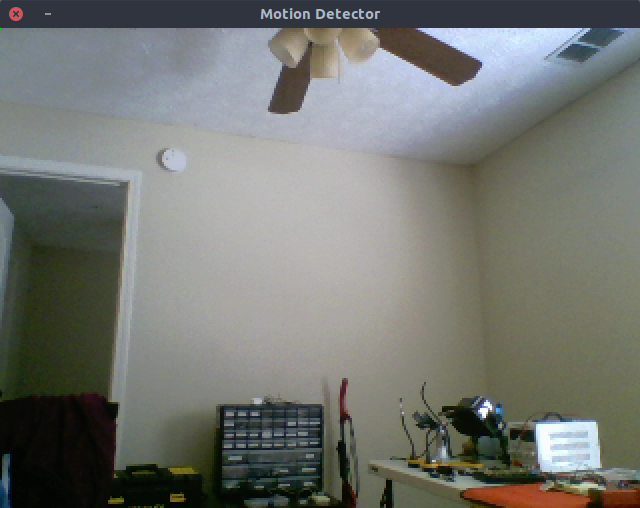
\includegraphics[width=2in]{startup.png}
    \caption{Motion Detector Program Window}
    \label{fig:startup_window}
    \end{minipage}

    \begin{minipage}{0.4\textwidth}
    \centering
    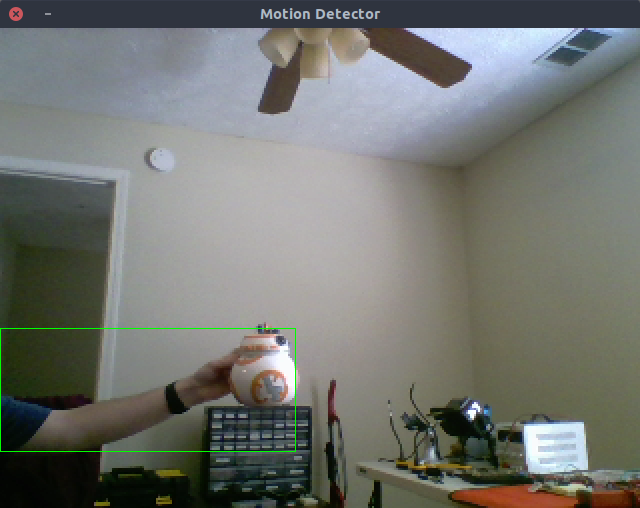
\includegraphics[width=2in]{motion.png}
    \caption{Motion Detector Program Window w/ Motion}
    \label{fig:motion_box}
    \end{minipage}
    
    \begin{minipage}{0.4\textwidth}
    \centering
    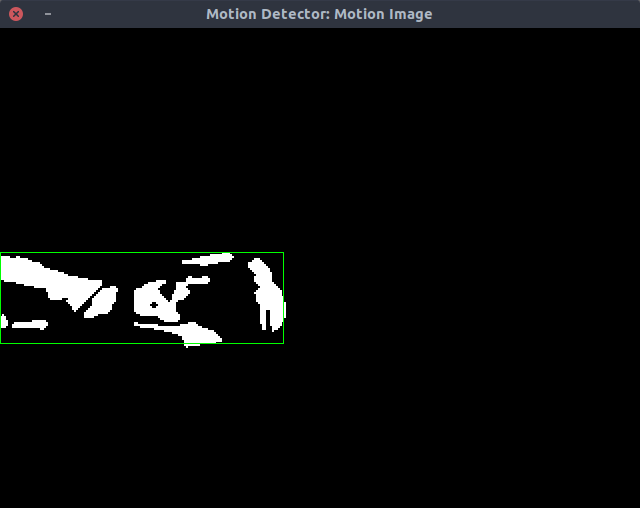
\includegraphics[width=2in]{motion_image.png}
    \caption{Motion Detector Program Window w/ Motion Image}
    \label{fig:motion_image}
    \end{minipage}
\end{figure}
\section{Tour of Implemented Program}
\label{section:program}
As stated in Section \ref{section:algorithm}, the program has two modes of operation, controlled back a compiler
flag. The first mode of operation is live motion detector that opens an actual video source and detects motion.
The second is an experiment mode that allows a series of images to be processed by the algorithm.

\subsection{Motion Detector Mode}
Motion Detector starts up and quickly creates a background model. Once the model is created a view of the scene
is presented as shown in \ref{fig:startup_window}. This a scaled up video feed of the webcam video. If motion
is detected, a green box is drawn around it as shown in Figure \ref{fig:motion_box}. Along with the webcam video,
this mode can also display the background model, motion image, and the motion mask. The views can be switched
between by pressing the "v" key on the keyboard. The title of the window is also updated to reflect the view
being displayed. Figure \ref{fig:motion_image} shows the example of a motion image.


\subsection{Testing Mode}
Testing model exposes the algorithm to allow for repeatable tests to be preformed. In this mode, arguments
are given to the location of the discrete frames to run through the algorithm. The motion image of each frame
is then output in a directory next to the source images. 

\section{Experiments}
\label{section:experiments}
Two types of experiments will be presented in this section. The first analyzes the performance 
of the algorithm and its ability to detect motion. The second looks at the computational 
performance and efficiency. 

\subsection{Motion Detection Results}
To preform repeatable experiments on real data, the \href{http://changedetection.net/}{CDNET} video 
database was used. CDNET has a wide collection of data sets of videos in different conditions and 
scenarios. The vidoesare gives as individual frames stored as JPEG images of a size 320x240.
They also provide a Matlab  program to score change detection algorithms off the data set.
While the algorithm proposed here is not a full change detection algorithm, this benchmark 
can still be used to provide some insight to its performance. The CDNET test expects an object 
to be fully colored in white if it is in motion. The parameters chosen to run these tests are 
shown in Table \ref{table:param}.

\begin{table}[h]
\caption{Algorithm Parameters}
\label{table:param}
\centering
\begin{tabular}{|l|l|}
\hline
Background Model Frame Size & 10  \\ \hline
Motion Threshold            & 225 \\ \hline
Filter Size                 & 3   \\ \hline
\end{tabular}
\end{table}

Table \ref{table:cdnet_score} shows the results of the algorithm on two datasets from CDNET chosen
from their resemblance to real surveillance video. The algorithm preformed very similarly between
the two data sets, both revving a precision rate of 12\%. Noth have a large number of False
negatives, this is caused by the error from the algorithm not filling in the full object in motion
and instead highlighting the edges of motion.

\begin{table}[t]
\centering
\caption{Algorithm Parameters}
\label{table:cdnet_score}
\begin{tabular}{|l|l|l|l|l|}
\hline
\textbf{Dataset} & \textbf{False Pos. Rate} & \textbf{False Neg. Rate} & \textbf{Precision} \\ \hline
Sofa & 0.78                     & 0.99                    & 0.12               \\ \hline
winterDriveway  & 0.73          & 1.00             & 0.12               \\ \hline
\end{tabular}
\end{table}


\subsubsection{Sofa Dataset}
The Sofa dataset is a video of a several men walking around and sitting on a sofa. Each man leaves something
in the scene before leaving it. It tests dynamic objects that become static background objects. Comparing a frame
where one of the men is walking to the corresponding motion image is shown is shown in Figure \ref{fig:man_capture} and Figure \ref{fig:man_motion} respectively. Viewing these two images, it is revealed
that a trail effect exists in behind the man. This occurs from capture being different from the background model
in those areas. The man was included in the background model, but as he continued to move an error was introduce. For motion detection in the context of this algorithm, this is acceptable.

\subsubsection{Winter Driveway}
The winter driveway data-set depicts a man waiting in a car in a snow covered driveway. He gets out and walks
around the car. There is also a lot of tree movement in the background. A sample frame and the corresponding 
motion map are shown in Figure \ref{fig:snow_man_capture} and Figure \ref{fig:snow_man_motion} respectively. The
trail effect is less noticeably here as the main is moving slowly between frames. As shown in this frame, 
the algorithm handles ignoring the moving trees pretty well. There are handful of frames with more tree
motion that causes some pixels to light up in the background. This data set also shows one weakness of
this algorithm. As the center part of the man is one fairly constant dark color, differences between frames
in this region are hard to detect. One way around this is to infer the shape of the man from the areas that
do change. As shown in this example and the example before, a clear outline is shown.

\begin{figure}[ht]
    \centering
    \begin{minipage}{0.4\textwidth}
    \centering
    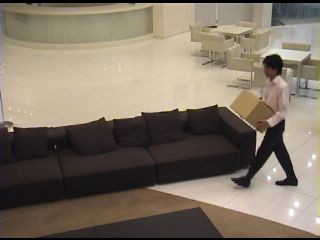
\includegraphics[width=2in]{in000113.jpg}
    \caption{Sofa: Capture of Man Walking}
    \label{fig:man_capture}
    \end{minipage}

    \begin{minipage}{0.4\textwidth}
    \centering
    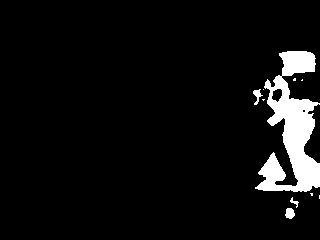
\includegraphics[width=2in]{bin000113.png}
    \caption{Sofe: Motion Image of Man Walking}
    \label{fig:man_motion}
    \end{minipage}
    
    \centering
    \begin{minipage}{0.4\textwidth}
    \centering
    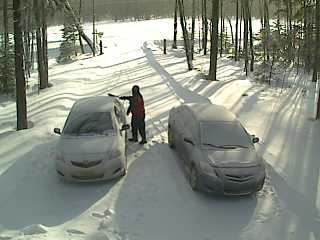
\includegraphics[width=2in]{in000554.jpg}
    \caption{Winter Driveway: Capture of Man Walking}
    \label{fig:snow_man_capture}
    \end{minipage}

    \begin{minipage}{0.4\textwidth}
    \centering
    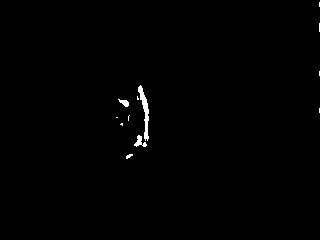
\includegraphics[width=2in]{bin000554.png}
    \caption{Winter Driveway: Motion Image of Man Walking}
    \label{fig:snow_man_motion}
    \end{minipage}
\end{figure}

\subsection{Computational Performance}

Figure \ref{table:preformance_table} shows the performance of the algorithm in testing mode. The tests were
preformed on a laptop with a Intel i7-4720HQ CPU at 2.60GHz. The execution time
only includes the time spent within the algorithm and does not include the time doing disk I/O to get and
save the frames. The frames per second of the algorithm was nearly constant around 47 FPS. This is expected
to remain the same as for each image of the same size, the number of computations required are exactly the same.

\begin{table}[ht]
\centering
\caption{Performance Comparison of the Algorithm}
\label{table:preformance_table}
\begin{tabular}{llll}
\cline{1-4}
\multicolumn{1}{|r|}{\textbf{Dataset}} & \multicolumn{1}{r|}{\textbf{Frames}} & \multicolumn{1}{r|}{\textbf{Execution Time (s)}} & \multicolumn{1}{r|}{\textbf{FPS}} \\ \cline{1-4}
\multicolumn{1}{|r|}{Sofa}             & \multicolumn{1}{r|}{2750}            & \multicolumn{1}{r|}{56.67}                       & \multicolumn{1}{r|}{48.52}  \\ \cline{1-4}
\multicolumn{1}{|r|}{Winter Driveway}  & \multicolumn{1}{r|}{2500}            & \multicolumn{1}{r|}{50.81}                       & \multicolumn{1}{r|}{48.20}  \\ \cline{1-4}
\multicolumn{1}{|r|}{Canoe}            & \multicolumn{1}{r|}{1189}            & \multicolumn{1}{r|}{26.22}                       & \multicolumn{1}{r|}{45.40}  \\ \cline{1-4}
\end{tabular}
\end{table}
Using the Linux tool \texttt{perf}, Table \ref{table:perf} shows the percent of time the program spends
in the top 8 functions of the algorithm. Unsurprisingly, smooth image is nearly half of the total computation
time. As its convolution is implemented in the image domain, it has to preform 691,200 multiplies for convolution
and find the median of each convolution window. \texttt{quick\_select}, which implements the median operation,
takes nearly 1/5 of the total processing time.

\begin{table}[ht]
\centering
\caption{Execution Time Percentages of Functions}
\label{table:perf}
\begin{tabular}{|l|c|}
\hline
\textbf{Function}            & \textbf{\% of Exec Time} \\ \hline
detect\_motion               & 100\%                                             \\ \hline
smooth\_image                & 51\%                                              \\ \hline
quick\_select                & 18\%                                              \\ \hline
yuv\_set\_pixel\_value       & 13\%                                              \\ \hline
magnitude                    & 9\%                                               \\ \hline
yuv\_get\_pixel\_value       & 7\%                                               \\ \hline
bg\_model\_get\_pixel\_value & 4\%                                               \\ \hline
bg\_model\_set\_pixel\_value & 3\%                                               \\ \hline
\end{tabular}
\end{table}

\section{Discussion}
\label{section:discussion}
The performance of the implementation is good enough to run a smooth 30FPS video feed on the development
computer. In order to implement this algorithm, some further optimizations should be made:

\subsection{Filtering}
The smoothing filter is this implementation is done in the image domain. Ideally, a Fast Fourier Transform
should be preformed and the convolution handled in the frequency domain. The \href{http://www.fftw.org/}{FFTW}
library implements DFFTs in C and has many optimizations options on cheaper ARM processors. The median filter should be removed and replaced with a cheaper filter to remove impulsive noises. Ideally 
something that can be one in the frequency domain.

\subsection{Motion Detection Performance}
The motion detector preformed fine in the context of simple video surveillance. Further efforts could be
explored to allow it to track multiple objects in motion at once. Efforts should also be take to eliminate
trailing effects and better fill in moving objects in the motion image.

\subsection{Threading and Other Optimizations}
When possible, threading could be employed here to divide and conquer the motion detection task. The image
could be broken up into sub-images which are then each processed on their own thread. Alternatively or
in-conjugation, GPU acceleration could be used to speed up the convolution.

\section{Conclusion}
Designing a motion detection algorithm for video surveillance is a trade off between computational performance 
and design performance. The algorithm presented in this report is simple to implement, and if optimized
properly, efficient for use in lower end systems. The algorithm presented in this report is functional on
the development hardware. The implementation presented needs further optimization. Utilizing optimizations 
techniques presented Section \ref{section:discussion}, may help mitigate this but not all optimizations are 
possible on lower end systems. Further testing would be need to prove the algorithm's performance
on these systems.

\appendices
\section{Code}
\label{appendix:code}
The code written for this project can be found on the project's  
\href{https://github.com/joeyahines/motion_detector}{Github Repo}. The code is written in C using \href{https://www.libsdl.org/}{SDL} for GUI rendering,  \href{https://www.linuxtv.org/downloads/v4l-dvb-apis-new/uapi/v4l/v4l2.html}{V4L}, \href{http://libjpeg.sourceforge.net/}{libjpeg} for JPEG image input, and \href{https://github.com/misc0110/libattopng}{libattopng} was ued to output PNG images. Code for capturing video was adapted from the \href{https://www.linuxtv.org/downloads/v4l-dvb-apis-new/uapi/v4l/capture.c.html}{Video Capture Example} in the V4L documentation. QuickSearch comes from an implementation defined in \cite{num_in_c}
The image manipulation and algorithm routines were written by me. 


% Can use something like this to put references on a page
% by themselves when using endfloat and the captionsoff option.
\ifCLASSOPTIONcaptionsoff
  \newpage
\fi



% trigger a \newpage just before the given reference
% number - used to balance the columns on the last page
% adjust value as needed - may need to be readjusted if
% the document is modified later
%\IEEEtriggeratref{8}
% The "triggered" command can be changed if desired:
%\IEEEtriggercmd{\enlargethispage{-5in}}

% references section

% can use a bibliography generated by BibTeX as a .bbl file
% BibTeX documentation can be easily obtained at:
% http://mirror.ctan.org/biblio/bibtex/contrib/doc/
% The IEEEtran BibTeX style support page is at:
% http://www.michaelshell.org/tex/ieeetran/bibtex/
\bibliographystyle{IEEEtran}
\bibliography{IEEEabrv,ref}

\end{document}
